\documentclass{sigchi}

% Use this section to set the ACM copyright statement (e.g. for
% preprints).  Consult the conference website for the camera-ready
% copyrights statement.

% Copyright
\CopyrightYear{2017}
%\setcopyright{acmcopyright}
\setcopyright{acmlicensed}
%\setcopyright{rightsretained}
%\setcopyright{usgov}
%\setcopyright{usgovmixed}
%\setcopyright{cagov}
%\setcopyright{cagovmixed}
% DOI
\doi{http://dx.doi.org/10.475/123_4}
% ISBN
\isbn{123-4567-24-567/08/06}
%Conference
\conferenceinfo{CHI'17,}{May 06--11, 2017, Denver, CO, USA}
%Price
\acmPrice{\$15.00}

% Use this command to override the default ACM copyright statement
% (e.g. for preprints).  Consult the conference website for the
% camera-ready copyright statement.

%% HOW TO OVERRIDE THE DEFAULT COPYRIGHT STRIP --
%% Please note you need to make sure the copy for your specific
%% license is used here!
% \toappear{
% Permission to make digital or hard copies of all or part of this work
% for personal or classroom use is granted without fee provided that
% copies are not made or distributed for profit or commercial advantage
% and that copies bear this notice and the full citation on the first
% page. Copyrights for components of this work owned by others than ACM
% must be honored. Abstracting with credit is permitted. To copy
% otherwise, or republish, to post on servers or to redistribute to
% lists, requires prior specific permission and/or a fee. Request
% permissions from \href{mailto:Permissions@acm.org}{Permissions@acm.org}. \\
% \emph{CHI '16},  May 07--12, 2016, San Jose, CA, USA \\
% ACM xxx-x-xxxx-xxxx-x/xx/xx\ldots \$15.00 \\
% DOI: \url{http://dx.doi.org/xx.xxxx/xxxxxxx.xxxxxxx}
% }

% Arabic page numbers for submission.  Remove this line to eliminate
% page numbers for the camera ready copy
% \pagenumbering{arabic}

% Load basic packages
\usepackage{balance}       % to better equalize the last page
\usepackage{graphics}      % for EPS, load graphicx instead 
\usepackage[T1]{fontenc}   % for umlauts and other diaeresis
\usepackage{txfonts}
\usepackage{mathptmx}
\usepackage[pdflang={en-US},pdftex]{hyperref}
\usepackage{color}
\usepackage{booktabs}
\usepackage{textcomp}


% Some optional stuff you might like/need.
\usepackage{microtype}        % Improved Tracking and Kerning
% \usepackage[all]{hypcap}    % Fixes bug in hyperref caption linking
\usepackage{ccicons}          % Cite your images correctly!
% \usepackage[utf8]{inputenc} % for a UTF8 editor only

% If you want to use todo notes, marginpars etc. during creation of
% your draft document, you have to enable the "chi_draft" option for
% the document class. To do this, change the very first line to:
% "\documentclass[chi_draft]{sigchi}". You can then place todo notes
% by using the "\todo{...}"  command. Make sure to disable the draft
% option again before submitting your final document.
\usepackage{todonotes}

% Paper metadata (use plain text, for PDF inclusion and later
% re-using, if desired).  Use \emtpyauthor when submitting for review
% so you remain anonymous.
\def\plaintitle{Design of an In-Home Educational Robot for Reading}
\def\plainauthor{Joseph E Michaelis, Bilge Mutlu}
\def\emptyauthor{}
\def\plainkeywords{Human-robot interaction; interest development; reading education; educational robotics}
\def\plaingeneralterms{Documentation, Standardization}

% llt: Define a global style for URLs, rather that the default one
\makeatletter
\def\url@leostyle{%
  \@ifundefined{selectfont}{
    \def\UrlFont{\sf}
  }{
    \def\UrlFont{\small\bf\ttfamily}
  }}
\makeatother
\urlstyle{leo}

% To make various LaTeX processors do the right thing with page size.
\def\pprw{8.5in}
\def\pprh{11in}
\special{papersize=\pprw,\pprh}
\setlength{\paperwidth}{\pprw}
\setlength{\paperheight}{\pprh}
\setlength{\pdfpagewidth}{\pprw}
\setlength{\pdfpageheight}{\pprh}

% Make sure hyperref comes last of your loaded packages, to give it a
% fighting chance of not being over-written, since its job is to
% redefine many LaTeX commands.
\definecolor{linkColor}{RGB}{6,125,233}
\hypersetup{%
  pdftitle={\plaintitle},
% Use \plainauthor for final version.
  pdfauthor={\plainauthor},
%  pdfauthor={\emptyauthor},
  pdfkeywords={\plainkeywords},
  pdfdisplaydoctitle=true, % For Accessibility
  bookmarksnumbered,
  pdfstartview={FitH},
  colorlinks,
  citecolor=black,
  filecolor=black,
  linkcolor=black,
  urlcolor=linkColor,
  breaklinks=true,
  hypertexnames=false
}

% create a shortcut to typeset table headings
% \newcommand\tabhead[1]{\small\textbf{#1}}

% End of preamble. Here it comes the document.
\begin{document}

\title{\plaintitle}

\numberofauthors{2}
\author{%
  \alignauthor{Leave Authors Anonymous\\
    \affaddr{for Submission}\\
    \affaddr{City, Country}\\
    \email{e-mail address}}\\
  \alignauthor{Leave Authors Anonymous\\
    \affaddr{for Submission}\\
    \affaddr{City, Country}\\
    \email{e-mail address}}\\
  %\alignauthor{Leave Authors Anonymous\\
   % \affaddr{for Submission}\\
    %\affaddr{City, Country}\\
    %\email{e-mail address}}\\
}

\maketitle

\begin{abstract}
  UPDATED---\today. Developing literacy and reading proficiency is considered an essential element of learning, and needs support in both the classroom and at home. However, little is known about how a robot might play a role in this development.  We used six specific design features based on recommendations from interest development and human-robot interaction literature to create an in-home learning companion robot. The robot was used as a technology probe to explore families' (N=8) current habits and views about reading, how a reading technology might be used, and how children percieved reading with the learning companion. Initial results indicate that reading with the learning companion may promote interest in reading, and was seen as a way to socially engage with reading and as a way to develop reading ability. We conclude with design recommendations and future work based on these findings.
  %139 words, 150 max
\end{abstract}

\category{H.5.m.}{Information Interfaces and Presentation
  (e.g. HCI)}{Miscellaneous} \category{See
  \url{http://acm.org/about/class/1998/} for the full list of ACM
  classifiers. This section is required.}{}{}

\keywords{\plainkeywords}

\section{Introduction}

Reading has long had an important and established place in education, and developing literacy and reading proficiency is considered a basic and essential element of learning \cite{McCormick:1994,Freire:1983}.  While classroom instruction for younger readers is an important part of this process, practicing and engaging with reading at home is also crucial for these students \cite{Baker:1997}.  With drastic technological advances in the last decade, the viability of using robots as educational agents to support learning, in both classrooms and in the home, has increased dramatically \cite{Benitti:2012}. These educational robots can act as learning companions, tutors,  or instructional agents and can provide individually tailored instruction to children \cite{Miller:2008}, and when used in the home, robots can support student learning and skill building to supplement classroom instruction. One type of instructional support that has proven beneficial to both learning outcomes and student engagement is the development of interest in a domain \cite{Hidi:2006}, and this support is especially useful for young readers \cite{Jones:2011}.  However, little is known about how an in-home learning companion robot might provide students with support for interest and engagement in reading. The goal of this study is to explore how young readers currently engage in reading at home and how they imagine technologies, such as robots, could enhance this; to observe how they interact with a robot designed as an in-home learning companion for reading; and to explore their beliefs about how they might use and benefit from a robot as a learning companion. To pursue these goals, we developed an in-home learning companion robot, Minnie, to use as a technology probe \cite{Hutchinson:2003}.

First, it is important to establish a rational for choosing a robot as the agent to provide reading support. Han, Jo, Park \& Kim \cite{Han:2005} were among the first to report on testing an educational robot for children in their homes. They found that a home robot promoted engagement, interest, and learning in English; and was also considered friendlier than other learning media. These increases may be due to a robot's ability to make better social connections and perform appropriate behavioral strategies than other computerized agents \cite{Brown:2013}, and social interactions have been found to positively influence interest in a task \cite{Sansone:2005}.  Other studies in human-robot interaction have found robots to be more engaging and life-like \cite{Kiesler:2008}, appealing, perceptive and helpful \cite{Wainer:2007}, and positive and natural \cite{Bainbridge:2011} than other computerized agents. This social nature of human-robot interaction motivates our use of a robot rather than a computerized agent as a learning companion for reading.

In this study we utilize research in interest development as well as in human-robot interactions to identify guidelines for supporting student engagement and interest in a reading task. Interest development researchers distinguish between situational interest,  a psychological state characterized by increased focus and attention, and individual interest, a predisposition to reengage with specific content \cite{Hidi:2006}.  It is believed that promoting situational interest by successfully \textit{triggering} (or catching), and then \textit{maintaining} (or holding) a student's interest during successive interactions can promote the development of emerging individual interest \cite{Hidi:2006, Mitchell:1993}. Guidelines for increasing catch and hold interest from this area of research include providing students with autonomy in choosing educational materials \cite{Jones:2011}; setting and monitoring reading goals \cite{Cabral:2015}; providig materials that align with student topic interests \cite{Ainley:2002} and that students believe they have the ability to be successful with; providing social partners who indicate interest in the activity \cite{Sansone:2005}, and reading out-loud to a social partner \cite{Rasinski:2003}. Findings from Human-Robot Interaction studies also provide several guidelines for increasing engagement during robot interactions, including: the robot making direct eye contact when speaking to an individual \cite{Mutlu:2011}; providing tailored recommendations for content \cite{Lim:2013}; expressing empathy \cite{Leite:2012}; and making reference to previous interactions \cite{Leite:2009}.

By utilizing these design guidelines we believe a robotic agent may be a powerful tool for supporting interest and engagement in reading for young readers. We have identified several specific features to be incorporated into a learning companion robot in order to promote student interest and engagement in reading. The first set of design guidelines involve the learning companion guiding students with reading, including: providing book recommendations based on topic interests, individual interest for reading, and feedback after completing a book; allowing the child to choose what book they read; and setting and monitoring reading time goals. Given that people have been found to interact with robots and other computerized agents in a social way \cite{Bickmore:2005}, the second set of design guidelines involve providing feedback and having social interactions with the children. These include: giving feedback that refers to previous interactions with the child; making eye contact with the child as they interact; and responding with detailed comments that empathize or otherwise relate to what the child is currently reading.

In this paper, we report on the use of Minnie, a robot designed with these guidelines, as a probe to gain a better understanding of how a learning companion robot may be used in a child's home, and how our design features will be perceived by the child and their family.  We begin with a description of how the robot is used as a technology probe, and how it was developed.  We then detail our data collection methods and results, discuss the implications of these results, and finally conclude with theoretical and practical contributions to both interest devleopment and human-robot interaction fields of research.


\section{METHOD}
 For this study, we first developed a learning companion robot, Minnie, based on our six design guidelines. In a manner inspired by Odom et. al \cite{Odom:2012}, we conducted short in-home visits with families to use the learning companion robot as a technology probe \cite{Hutchinson:2003} for discussion and reflection on how a reading technology might impact current reading habits in each home.  Hutchinson et. al \cite{Hutchinson:2003} describes the technology probe approach as a method with three goals: understanding the user's needs and feelings about the technology, field-testing a technology, and reflection on new possibilites for the technology.  These goals are in-line with our aim for this study in that we believe that at this stage of development our prior understanding of the intended user may not be sufficient, which may limit our view of how and what the learning companion robot should do. The introduction of the learning companion into the home may inspire new thoughts and possibilities on it's use, and we intend to explore these and make modifications prior to empirical testing of the design. Thus, our field testing of the robot should be concurrent to deep exploration of the design space through the eyes of the user.  
 
 We began the in-home visit by asking one child (referred to after as the \textit{main child} to complete a short individual interest in reading survey, followed by an interview (pre-) with the family.  After the pre-interview, we introduced our learning companion robot to the family and asked the main child in the home to interact with it. Following the interaction, we asked the main child to complete another short survey, this time about their situational interest for the interact.  Finally, we completed a second interview (post-) with the family. In the spirit of using the technology as a probe, we did not limit the discussion or interaction with the robot to our preconceived ideas about how, when and where the learning companion should and would be used. Rather, we allowed families to explore ideas about how they would like to or would use this or another technology for reading. The following describes this method in more detail.
 
\subsection{Design of the Robot}
Our initail design of the learning companion robot was guided by a desire to leverage the power of social interaction to promote interest and engagement in reading.  In our view a small, desktop humanoid robot with multiple methods of interaction and non-verbal expression would be appropriate.  We also felt that the robot should be built on a simple, modifiable, and inexpensive platform in order to model the type of constraints inherent in an affordable commericially available robot, and allow for hardware modifications.  This intuition led us to create the robot using a modified version of a freely available 3D printable robot design from Hello Robo \cite{Robo:2016}.  A more expensive pre-made robot such as the popular Nao platform, while possibly more reliable and polished, is not flexible in it's physical and hardward design.  

The original robot from Hello Robo stands 13.5 inches and has a static torso without any movable appendages (see Figure 1).  The head and neck of the robot contain five servo controlled motions including: two closing eyelids, a pair of eyes that move laterally together, and vertical and horizontal head movements.  These motion options allowed us to create specific robot behaviors to provide a life-like feel (e.g. blinking eyes), and non-verbal communication (e.g. looking directly at a person).  Our modifications to the original robot included adding three pieces of hardware to the robot in order to facilitate human-robot communcation. First, we embedded a speaker in each of the ear pieces to allow the robot to utilize text-to-speech responses to the child.  Second, we included an RFID reader in the lower front of the robot to allow the child to respond to the robot with four color coded, pre-programmed RFID cards.  Roughly, the cards allow the child to \textit{say} yes/continue, no/stop, pause, and repeat to the robot.  Third, we added a USB camera to achieve two purposes: allowing video input to process facial recognition, which we used for facial tracking; and reading visual tags (AprilTags; \cite{}) placed within books.  The robot hardware design allows us to implement the six design features we identified from our literature review.

\begin{figure}
	\centering
	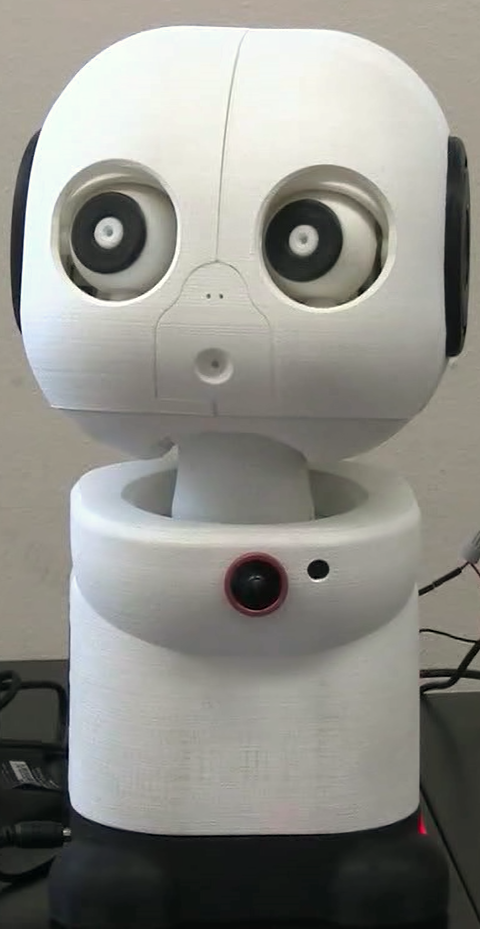
\includegraphics[width=0.6\columnwidth]{figures/minnie}
	\caption{Image of the learning compantion robot, Minnie, used in the study.  The camera is the red circle on the upper torso.  The RFID reader is below the camera. }~\label{fig:figure1}
\end{figure}

\subsection{Robot Interaction}
After completing the interview, the main child was introduced to the learning companion robot, and was asked where in their home they would likely read with the robot.  Of the suggestions made by the child, we asked the parent(s) which of these areas they would be most comfortable with us conducting the robot interaction, and chose to work there.  In this way, we were able to allow for as authentic of an interaction between the child and robot, while maintaining the comfort and trust of the parent. 

\subsection{Participants}
 We recruited families (N=8) from a mid-sized midwestern city to participate in the study. Most often one parent and one child participated, while one family included two parents, and two families had one younger sibling present. For each family, one main child (mean age = 11.6; age range: 11 - 12; male = 5) was asked to interact directly with the learning companion robot.  All other family members were included in pre- and post-interviews.
 
  
\subsection{Data Sources}
  During the course of our study, we collected data from three major sources.  The first type of data source were three separate surveys.  One survey was completed by parents as pre-visit questionairre on their child's reading ability and habits.  The other two were completed by the main child: an individual interest in reading survey prior to working with the learning companion robot, and a situational interest survey after.  Reliability for the individual and situational interest scales was measured using Cronbach’s alpha, with an alpha value of 0.7 or greater indicating, by convention, a reasonably reliable construct \cite{Crocker:2009}.  The second data source was from transcriptions of video recorded semi-structured inteviews conducted before (pre-) and after (post-) the robot interaction. Both interviews were approximately 15 - 20 minutes in lenght, with the pre-interview (\textit{M} = \#\#\# minutes, \textit{SD} = \#\#\# minutes) being slightly longer than the post-interview (\textit{M} = \#\#\# minutes, \textit{SD} = \#\#\# minutes). Finally, the third data source comes from coding segements of video recordings made during the robot intereaction of about 30 minutes (\textit{M} = \#\#\# minutes, \textit{SD} = \#\#\# minutes)).  The following discusses each data source in more detail.
  
\subsubsection{Survey}

  Prior to the in-home visit one parent for each family was asked to complete a questionairre to collect some information about the main child.  We asked the parent to describe, to the best of their knowledge, their child's reading ability, the amount of time their child spends reading non-school work each week, their (the parent's) satisfaction with the amount of time their child spends reading, as well as some basic demographic information (e.g. age and grade).
  
  During the in-home visit, the main child was first asked to complete a 10-item pre-survey to assess the child's individual interest in reading.  This survey was developed by rewording items from the Four-Phase Interest in Engineering Survey (FIDES) by Michaelis \& Nathan \cite{Michaelis:2015} with the reading motivation language in the Motivation for Reading Questionairre by Wigfield \& Guthrie \cite{Wigfield:1997}. The survey is comprised of Likert-style items, which asked students to rate their level of agreement with statements using a scale from 1 (\textit{strongly disagree}) to 7 (\textit{strongly agree}). Scores were calculated by averaging a sum of scores from all items to produce scores on the 1 to 7 Likert scale equivalent (Mean = ). The high Cronbach\text{'}s alpha ($\alpha$ = \#\#\#) indicates it has a high internal reliability.
  
  After engaging with the learning companion robot, the child was asked to complete a post-survey with six Likert-style items, using the same 1 to 7 scale, to assess the child's level of catch (3 items) and hold (3 items) situational interest during the reading activity.  The survey was based on prior work by Knogler, Harackiewicz, Gegenfurtner, and Lewalter \cite{Knogler:2015}.  Scores were averaged for catch (Mean = ) and hold (Mean = )items to produce scores on the 1 to 7 Likert scale equivalent. Cronbach\text{'}s alphas were calculated separately for catch ($\alpha$ = \#\#\#) and hold ($\alpha$ = \#\#\#) scales, and both values indicated a highly reliable scale.  
  
\subsubsection{Interview and Robot Interaction}
  Two sources of video data were analyized for the study: two interviews with the family (pre- and post-), and the main child's interaction with the robot. For the semi-structured interviews, a pre-determined set of questions was used as a focus for the interaction.  However, the researcher pursued ideas from the family members in a conversational style, and encouraged them to elaborate and explain their thinking. The pre- and post- interviews were both transcribed verbatim and segemented by distinct ideas \cite{Chi:1997}.
  
  We video recorded a semi-structured pre-interview with the family about their current reading habits (e.g. How often do you read?); what motivates their child to read (e.g. What systems do you have in place to encourage your child to read?); and the family's familiarity, experience, and thoughts about working with technology for reading (e.g. If you had a technology that worked with you while you read, what would it do?). After the pre-interview, the main child was introduced to the robot, and instructed on how to begin working with the robot.  Once they were ready to begin we video recorded the entirety of their interaction. After the robot interaction was completed, and a short situational interest survey was administered, we conducted a second semi-structured interview (post-) with the family.  This interview was about the family memebers' view of the robot as a partner (e.g. Did it feel like Minnie was alive?), their likes and dislikes about the robot interaction (e.g. Are there any things you would change about Minnie?), and whether they thought the robot would be a useful tool for the home (e.g. If the robot were released to the market today, would you be interested in  buying one for your child?)
  
  All video data was coded using a Grounded Theory approach. In using a Grounded Theory analysis we begin with an open coding period where emerging themes were identified and defined as codes.  These codes are then applied to important statements, segments, or ideas from the transcripts.  After initial codes were identified and applied, the reliability of these codes was examined by comparing inter-rater reliability on 10\% of the data.  The inter-rater reliability was very high between coders for both pre- ($\kappa$ = \#\#\#) and post-interviews  ($\kappa$ = \#\#\#), as well for the robot interaction videos ($\kappa$ = \#\#\#).  We then developed axial codes for each data set to further refine our coding scheme into related categories, and then finally developed a third level of coding of major themes of our findings, which expressed relationships between the axial codes.  In total we 
 
\section{Findings}
The styles contained in this document have been modified from the
default styles to reflect ACM formatting conventions. For example,
content paragraphs like this one are formatted using the Normal style.

\LaTeX\ sometimes will create overfull lines that extend into columns.
To attempt to combat this, the \texttt{.cls} file has a command,
\texttt{{\textbackslash}sloppy}, that essentially asks \LaTeX\ to
prefer underfull lines with extra whitespace.  For more details on
this, and info on how to control it more finely, check out
{\url{http://www.economics.utoronto.ca/osborne/latex/PMAKEUP.HTM}}.


\subsection{Title and Authors}

Your paper's title, authors and affiliations should run across the
full width of the page in a single column 17.8 cm (7 in.) wide.  The
title should be in Helvetica or Arial 18-point bold.  Authors' names
should be in Times New Roman or Times Roman 12-point bold, and
affiliations in 12-point regular.  

See \texttt{{\textbackslash}author} section of this template for
instructions on how to format the authors. For more than three
authors, you may have to place some address information in a footnote,
or in a named section at the end of your paper. Names may optionally
be placed in a single centered row instead of at the top of each
column. Leave one 10-point line of white space below the last line of
affiliations.

\subsection{Abstract and Keywords}

Every submission should begin with an abstract of about 150 words,
followed by a set of Author Keywords and ACM Classification
Keywords. The abstract and keywords should be placed in the left
column of the first page under the left half of the title. The
abstract should be a concise statement of the problem, approach, and
conclusions of the work described. It should clearly state the paper's
contribution to the field of HCI\@.

\subsection{Normal or Body Text}

Please use a 10-point Times New Roman or Times Roman font or, if this
is unavailable, another proportional font with serifs, as close as
possible in appearance to Times Roman 10-point. Other than Helvetica
or Arial headings, please use sans-serif or non-proportional fonts
only for special purposes, such as source code text.

\subsection{First Page Copyright Notice}
This template include a sample ACM copyright notice at the bottom of
page 1, column 1.  Upon acceptance, you will be provided with the
appropriate copyright statement and unique DOI string for publication.
Accepted papers will be distributed in the conference
publications. They will also be placed in the ACM Digital Library,
where they will remain accessible to thousands of researchers and
practitioners worldwide. See
\url{http://acm.org/publications/policies/copyright_policy} for the
ACM's copyright and permissions policy.

\subsection{Subsequent Pages}

On pages beyond the first, start at the top of the page and continue
in double-column format.  The two columns on the last page should be
of equal length.



\subsection{References and Citations}

Use a numbered list of references at the end of the article, ordered
alphabetically by last name of first author, and referenced by numbers
in
brackets~\cite{Han:2005}.
Your references should be published materials accessible to the
public. Internal technical reports may be cited only if they are
easily accessible (i.e., you provide the address for obtaining the
report within your citation) and may be obtained by any reader for a
nominal fee. Proprietary information may not be cited. Private
communications should be acknowledged in the main text, not referenced
(e.g., ``[Borriello, personal communication]'').

References should be in ACM citation format:
\url{http://acm.org/publications/submissions/latex_style}. This
includes citations to internet
resources~\cite{Han:2005}
according to ACM format, although it is often appropriate to include
URLs directly in the text, as above.


% Use a numbered list of references at the end of the article, ordered
% alphabetically by first author, and referenced by numbers in
% brackets~\cite{ethics, Klemmer:2002:WSC:503376.503378,
%   Mather:2000:MUT, Zellweger:2001:FAO:504216.504224}. For papers from
% conference proceedings, include the title of the paper and an
% abbreviated name of the conference (e.g., for Interact 2003
% proceedings, use \textit{Proc. Interact 2003}). Do not include the
% location of the conference or the exact date; do include the page
% numbers if available. See the examples of citations at the end of this
% document. Within this template file, use the \texttt{References} style
% for the text of your citation.

% Your references should be published materials accessible to the
% public.  Internal technical reports may be cited only if they are
% easily accessible (i.e., you provide the address for obtaining the
% report within your citation) and may be obtained by any reader for a
% nominal fee.  Proprietary information may not be cited. Private
% communications should be acknowledged in the main text, not referenced
% (e.g., ``[Robertson, personal communication]'').

\begin{table}
  \centering
  \begin{tabular}{l r r r}
    % \toprule
    & & \multicolumn{2}{c}{\small{\textbf{Test Conditions}}} \\
    \cmidrule(r){3-4}
    {\small\textit{Name}}
    & {\small \textit{First}}
      & {\small \textit{Second}}
    & {\small \textit{Final}} \\
    \midrule
    Marsden & 223.0 & 44 & 432,321 \\
    Nass & 22.2 & 16 & 234,333 \\
    Borriello & 22.9 & 11 & 93,123 \\
    Karat & 34.9 & 2200 & 103,322 \\
    % \bottomrule
  \end{tabular}
  \caption{Table captions should be placed below the table. We
    recommend table lines be 1 point, 25\% black. Minimize use of
    table grid lines.}~\label{tab:table1}
\end{table}

\section{Sections}

The heading of a section should be in Helvetica or Arial 9-point bold,
all in capitals. Sections should \textit{not} be numbered.

\subsection{Subsections}

Headings of subsections should be in Helvetica or Arial 9-point bold
with initial letters capitalized.  For sub-sections and
sub-subsections, a word like \emph{the} or \emph{of} is not
capitalized unless it is the first word of the heading.

\subsubsection{Sub-subsections}

Headings for sub-subsections should be in Helvetica or Arial 9-point
italic with initial letters capitalized.  Standard
\texttt{{\textbackslash}section}, \texttt{{\textbackslash}subsection},
and \texttt{{\textbackslash}subsubsection} commands will work fine in
this template.

\section{Figures/Captions}

Place figures and tables at the top or bottom of the appropriate
column or columns, on the same page as the relevant text (see
Figure~\ref{fig:figure1}). A figure or table may extend across both
columns to a maximum width of 17.78 cm (7 in.).

\begin{figure*}
  \centering
  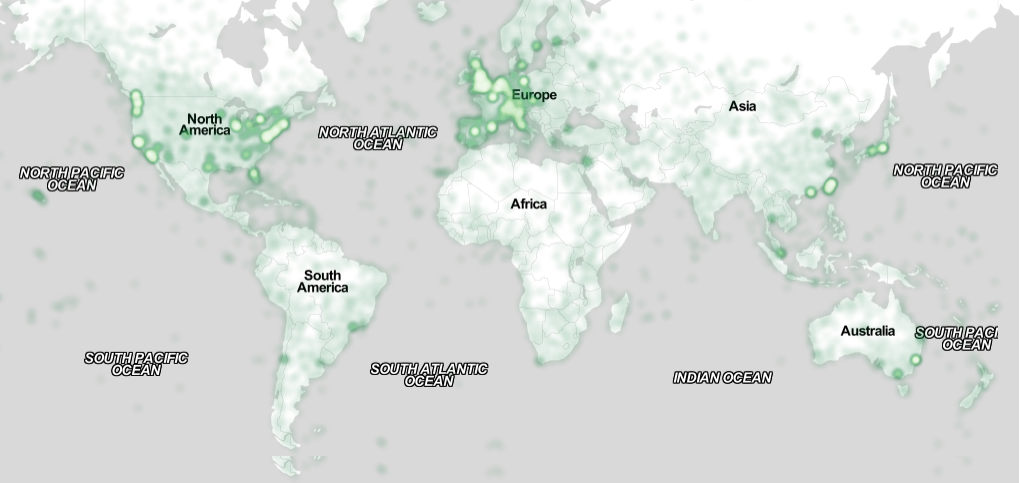
\includegraphics[width=1.75\columnwidth]{figures/map}
  \caption{In this image, the map maximizes use of space. You can make
    figures as wide as you need, up to a maximum of the full width of
    both columns. Note that \LaTeX\ tends to render large figures on a
    dedicated page. Image: \ccbynd~ayman on
    Flickr.}~\label{fig:figure2}
\end{figure*}

Captions should be Times New Roman or Times Roman 9-point bold.  They
should be numbered (e.g., ``Table~\ref{tab:table1}'' or
``Figure~\ref{fig:figure1}''), centered and placed beneath the figure
or table.  Please note that the words ``Figure'' and ``Table'' should
be spelled out (e.g., ``Figure'' rather than ``Fig.'') wherever they
occur. Figures, like Figure~\ref{fig:figure2}, may span columns and
all figures should also include alt text for improved accessibility.
Papers and notes may use color figures, which are included in the page
limit; the figures must be usable when printed in black-and-white in
the proceedings.

The paper may be accompanied by a short video figure up to five
minutes in length. However, the paper should stand on its own without
the video figure, as the video may not be available to everyone who
reads the paper.  

\subsection{Inserting Images}
When possible, include a vector formatted graphic (i.e. PDF or EPS).
When including bitmaps,  use an image editing tool to resize the image
at the appropriate printing resolution (usually 300 dpi).

\section{Quotations}
Quotations may be italicized when \textit{``placed inline''} (Anab,
23F).

\begin{quote}
Longer quotes, when placed in their own paragraph, need not be
italicized or in quotation marks when indented (Ramon, 39M).  
\end{quote}

\section{Language, Style, and Content}

The written and spoken language of SIGCHI is English. Spelling and
punctuation may use any dialect of English (e.g., British, Canadian,
US, etc.) provided this is done consis- tently. Hyphenation is
optional. To ensure suitability for an international audience, please
pay attention to the following:

\begin{itemize}
\item Write in a straightforward style.
\item Try to avoid long or complex sentence structures.
\item Briefly define or explain all technical terms that may be
  unfamiliar to readers.
\item Explain all acronyms the first time they are used in your
  text---e.g., ``Digital Signal Processing (DSP)''.
\item Explain local references (e.g., not everyone knows all city
  names in a particular country).
\item Explain ``insider'' comments. Ensure that your whole audience
  understands any reference whose meaning you do not describe (e.g.,
  do not assume that everyone has used a Macintosh or a particular
  application).
\item Explain colloquial language and puns. Understanding phrases like
  ``red herring'' may require a local knowledge of English.  Humor and
  irony are difficult to translate.
\item Use unambiguous forms for culturally localized concepts, such as
  times, dates, currencies, and numbers (e.g., ``1--5--97'' or
  ``5/1/97'' may mean 5 January or 1 May, and ``seven o'clock'' may
  mean 7:00 am or 19:00). For currencies, indicate equivalences:
  ``Participants were paid {\fontfamily{txr}\selectfont \textwon}
  25,000, or roughly US \$22.''
\item Be careful with the use of gender-specific pronouns (he, she)
  and other gendered words (chairman, manpower, man-months). Use
  inclusive language that is gender-neutral (e.g., she or he, they,
  s/he, chair, staff, staff-hours, person-years). See the
  \textit{Guidelines for Bias-Free Writing} for further advice and
  examples regarding gender and other personal
  attributes. Be particularly aware of
  considerations around writing about people with disabilities.
\item If possible, use the full (extended) alphabetic character set
  for names of persons, institutions, and places (e.g.,
  Gr{\o}nb{\ae}k, Lafreni\'ere, S\'anchez, Nguy{\~{\^{e}}}n,
  Universit{\"a}t, Wei{\ss}enbach, Z{\"u}llighoven, \r{A}rhus, etc.).
  These characters are already included in most versions and variants
  of Times, Helvetica, and Arial fonts.
\end{itemize}

\section{Accessibility}
The Executive Council of SIGCHI has committed to making SIGCHI
conferences more inclusive for researchers, practitioners, and
educators with disabilities. As a part of this goal, the all authors
are asked to work on improving the accessibility of their
submissions. Specifically, we encourage authors to carry out the
following five steps:
\begin{enumerate}
\item Add alternative text to all figures
\item Mark table headings
\item Add tags to the PDF
\item Verify the default language
\item Set the tab order to ``Use Document Structure''
\end{enumerate}
For more information and links to instructions and resources, please
see: \url{http://chi2016.acm.org/accessibility}.  The
\texttt{{\textbackslash}hyperref} package allows you to create well tagged PDF files,
please see the preamble of this template for an example.

\section{Page Numbering, Headers and Footers}
Your final submission should not contain footer or header information
at the top or bottom of each page. Specifically, your final submission
should not include page numbers. Initial submissions may include page
numbers, but these must be removed for camera-ready. Page numbers will
be added to the PDF when the proceedings are assembled.

\section{Producing and Testing PDF Files}

We recommend that you produce a PDF version of your submission well
before the final deadline.  Your PDF file must be ACM DL
Compliant. The requirements for an ACM Compliant PDF are available at:
{\url{http://www.sheridanprinting.com/typedept/ACM-distilling-settings.htm}}.

Test your PDF file by viewing or printing it with the same software we
will use when we receive it, Adobe Acrobat Reader Version 10. This is
widely available at no cost. Note that most
reviewers will use a North American/European version of Acrobat
reader, so please check your PDF accordingly.

When creating your PDF from Word, ensure that you generate a tagged
PDF from improved accessibility. This can be done by using the Adobe
PDF add-in, also called PDFMaker. Select Acrobat | Preferences from
the ribbon and ensure that ``Enable Accessibility and Reflow with
tagged Adobe PDF'' is selected. You can then generate a tagged PDF by
selecting ``Create PDF'' from the Acrobat ribbon.

\section{Conclusion}

It is important that you write for the SIGCHI audience. Please read
previous years' proceedings to understand the writing style and
conventions that successful authors have used. It is particularly
important that you state clearly what you have done, not merely what
you plan to do, and explain how your work is different from previously
published work, i.e., the unique contribution that your work makes to
the field. Please consider what the reader will learn from your
submission, and how they will find your work useful. If you write with
these questions in mind, your work is more likely to be successful,
both in being accepted into the conference, and in influencing the
work of our field.

\section{Acknowledgments}

Sample text: We thank all the volunteers, and all publications support
and staff, who wrote and provided helpful comments on previous
versions of this document. Authors 1, 2, and 3 gratefully acknowledge
the grant from NSF (\#1234--2012--ABC). \textit{This whole paragraph is
  just an example.}

% Balancing columns in a ref list is a bit of a pain because you
% either use a hack like flushend or balance, or manually insert
% a column break.  http://www.tex.ac.uk/cgi-bin/texfaq2html?label=balance
% multicols doesn't work because we're already in two-column mode,
% and flushend isn't awesome, so I choose balance.  See this
% for more info: http://cs.brown.edu/system/software/latex/doc/balance.pdf
%
% Note that in a perfect world balance wants to be in the first
% column of the last page.
%
% If balance doesn't work for you, you can remove that and
% hard-code a column break into the bbl file right before you
% submit:
%
% http://stackoverflow.com/questions/2149854/how-to-manually-equalize-columns-
% in-an-ieee-paper-if-using-bibtex
%
% Or, just remove \balance and give up on balancing the last page.
%
\balance{}

\section{References Format}
Your references should be published materials accessible to the
public. Internal technical reports may be cited only if they are
easily accessible and may be obtained by any reader for a nominal
fee. Proprietary information may not be cited. Private communications
should be acknowledged in the main text, not referenced (e.g.,
[Golovchinsky, personal communication]). References must be the same
font size as other body text. References should be in alphabetical
order by last name of first author. Use a numbered list of references
at the end of the article, ordered alphabetically by last name of
first author, and referenced by numbers in brackets. For papers from
conference proceedings, include the title of the paper and the name of
the conference. Do not include the location of the conference or the
exact date; do include the page numbers if available. 

References should be in ACM citation format:
\url{http://www.acm.org/publications/submissions/latex_style}.  This
includes citations to Internet
resources according to ACM format, although it is often appropriate to include
URLs directly in the text, as above. Example reference formatting for
individual journal articles, articles in conference
proceedings is given here.  See the examples of
citations at the end of this document and in the accompanying
\texttt{BibTeX} document. This formatting is a edited version of the
format automatically generated by the ACM Digital Library
(\url{http://dl.acm.org}) as ``ACM Ref.'' DOI and/or URL links are
optional but encouraged as are full first names. Note that the
Hyperlink style used throughout this document uses blue links;
however, URLs in the references section may optionally appear in
black.

% BALANCE COLUMNS
\balance{}

% REFERENCES FORMAT
% References must be the same font size as other body text.
\bibliographystyle{SIGCHI-Reference-Format}
\bibliography{chi17-michaelis}

\end{document}

%%% Local Variables:
%%% mode: latex
%%% TeX-master: t
%%% End:
